\section{Overview}\label{sec:ep}

\begin{figure}[tbp]
\centering
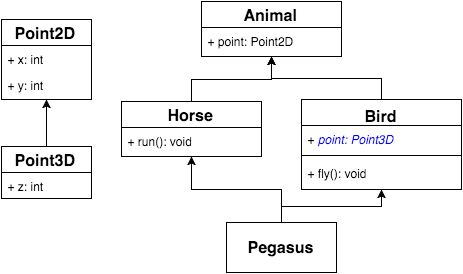
\includegraphics[width=4in]{PegasusDetail.png}
\caption{Pegasus Example.}\label{fig:pegasus}
\end{figure}

\subsection{A Running Example: Animals}
Suppose we want to model an animal system as shown in Fig~\ref{fig:pegasus}. In
order to model \texttt{Pegasus}, \emph{multiple inheritance} is clearly needed
in this example. Therefore, in Java we use interfaces instead of classes. An
\texttt{Animal} has a \texttt{point} field, indicating the current position of
the animal. \texttt{Horse} and \texttt{Bird} are subtypes of \texttt{Animal},
with methods \texttt{run()} and \texttt{fly()}, respectively. Note that
\texttt{Bird} can fly, therefore refines the type of \texttt{point} from
\texttt{Point2D} to \texttt{Point3D}. Pegasus (one of the best known creatures
in Greek mythology) can not only \emph{run} but also \emph{fly}! This is the
place where \emph{``multiple inheritance''} is needed, because \texttt{Pegasus}
need to obtain \texttt{fly} and \texttt{run} functionality from both
\texttt{Horse} and \texttt{Bird}.

\subsubsection{Model field members and constructors}
Firstly, to model \texttt{Point2D} that has x-coordinate and y-coordinate by an
interface, we immediately run into the problem of expressing the fields
\texttt{x} and \texttt{y}. Since in Java there is no way to define member fields
inside interfaces, we propose to simulate fields by abstract methods inside
interfaces. Method \texttt{withX, withY} creates a new instance of
\texttt{Point2D} with updated field \texttt{x,y}, respectively.

% Firstly, to model \texttt{Animal} by an interface, we immediately run into the
% problem of expressing the field \texttt{point}. Since in Java there is no way to
% define member fields inside interfaces, we propose to simulate fields by
% abstract methods inside interfaces:

\lstinputlisting[linerange=46-52]{../UseMixinLombok/src/test/TestAnimal.java}% APPLY:linerange=POINT2D

\paragraph{Instantiation}
In Java, to implement an interface like \texttt{Point2D}, a typical and trivial
approach that programmers usually do is creating a class extending the interface
and providing implementation for all methods inside. For example, this is the
implementation for interface \texttt{Point2D}:

\begin{lstlisting}
class Point2DImpl implements Point2D {
    private int _x;
    private int _y;
    public Point2DImpl(int x, int y) {
        this._x = x;
        this._y = y;
    }
    public int x() {
        return _x;
    }
    public int y() {
        return _y;
    }
    public Point2D withX(int x) {
        x(x);
        return this;
    }
    public void x(int x) {
        _x = x;
    }
    public void y(int y) {
        _y = y;
    }
    public Point2D withY(int y) {
        y(y);
        return this;
    }
}
\end{lstlisting}

\texttt{Point2DImpl} implements \texttt{Point2D} and provides a constructor with
quite mechanical code. What's worse, the implementation in \texttt{Point2DImpl}
may not be reused in a single inheritance language.

\paragraph{Our Approach}
Instead of writing a whole another class to provide the implementation for
\texttt{Point2D}, we annotate on interface \texttt{Point2D} directly with
\mixin. The \mixin annotation will generate a static method \texttt{of} inside
the interface. The \texttt{of} method mimics the functionality of constructors,
it takes arguments same as constructors and return objects similar to
constructors. It makes use of Java anonymous classes and achieves the same
implementation as \texttt{Point2DImpl}.

With our approach, we provide a Java annotation \mixin to provide default
implementations for various methods (e.g. getters, setters, with-methods, etc)
and a mechanism to instantiate objects. \mixin annotation helps programmers to
write less cumbersome code and instantiate interfaces in Java.

\begin{lstlisting}
  // inside interface Point2D
  static Point of(int x, int y) {
      return new Point() {
          int _x = x;
          int _y = y;
          public int x() {
            return _x;
          }
          public int y() {
            return _y;
          }
          public Point2D withX(int x) {
            x(x);
            return this;
          }
          public void x(int x) {
            _x = x;
          }
          public void y(int y) {
            _y = y;
          }
          public Point2D withY(int y) {
            y(y);
            return this;
          }
    }
  }
\end{lstlisting}

%\lstinputlisting[linerange=15-27]{../UseMixinLombok/src/overview/TestPoint.java} % APPLY:linerange=POINT_OF

\subsubsection{Model concrete methods}
Now we proceed to define \texttt{Animal} with \texttt{point} ``member
field''. Again, we model this member field with getter and setter methods:
\lstinputlisting[linerange=64-67]{../UseMixinLombok/src/test/TestAnimal.java}% APPLY:linerange=ANIMAL
\lstinputlisting[linerange=71-76]{../UseMixinLombok/src/test/TestAnimal.java}% APPLY:linerange=HORSE

For interface \texttt{Horse}, concrete implementation of \texttt{run()} method
need to be defined. Before Java 8, concrete methods (except for static methods)
are not allowed to appear in interfaces as in classes. But Java 8 introduces
\emph{default methods}, which allow for implementation insides interfaces. We
are making use of default methods to implement \texttt{run()}.  Interface also
\texttt{Horse} shows the usage and advantage of \emph{with} methods by method
\texttt{run()}: method \texttt{withX} returns a new point object with field
\texttt{x} updated by the argument to \texttt{withX}. Without these
\texttt{with} methods, operations like \texttt{run()} would be much harder to
define.

\subsubsection{Type Refinement}
\texttt{Bird} needs a 3D position, thus we define \texttt{Point3D} and
\texttt{Bird} as follows:
\lstinputlisting[linerange=56-60]{../UseMixinLombok/src/test/TestAnimal.java}% APPLY:linerange=POINT3D
\lstinputlisting[linerange=80-92]{../UseMixinLombok/src/test/TestAnimal.java}% APPLY:linerange=BIRD

Interface \texttt{Point3D} extends \texttt{Point2D} with a new abstract method
\texttt{int z()} (treated as a getter for member field \texttt{z}). Note that
the return type of various methods (e.g. with- methods, getters) get refined
either by covariant method overriding or automatically by our annotation
processor. Besides \emph{with}, other methods (including \emph{clone},
\emph{of}) also do type-refinements automatically.

\subsubsection{Multiple Inheritance}
The \emph{``multiple inheritance''} case appears at interface
\texttt{Pegasus}. Pegasuses can not only \emph{run} but also \emph{fly}!
Interface \texttt{Pegasus} obtains \texttt{fly} and \texttt{run} functionality
through interface \texttt{Horse} and \texttt{Bird}. Using \mixin annotation,
actually these is no code at all programmers have to write. The idea of using
default methods inside interfaces was proposed in ~\cite{}. It enables us to do
multiple inheritance, which otherwise is hard to do in Java-like languages that
do not support multiple inheritance, easily.

\lstinputlisting[linerange=96-97]{../UseMixinLombok/src/test/TestAnimal.java}% APPLY:linerange=PEGASUS

\begin{comment}
\subsection{A Running Example: \texttt{Point}}
Suppose we want to create a point component that models the a point in space,
that has x-coordinate and y-coordinate. For example, if we create the
\texttt{Point} interface in Java, it would look like this:

\begin{lstlisting}
interface Point {
    int x();
    int y(); 
}
\end{lstlisting}

\texttt{Point} has two (conceptually) member fields \texttt{x} and \texttt{y},
representing the two coordinates of a point. Methods \texttt{int x()} and
\texttt{int y()} serve as \emph{getter} methods. 
% Methods \texttt{void X(int X)} and \texttt{void Y(int Y)} serve as
% \emph{setter} methods. Method \texttt{Point withX(int X)} updates field
% \texttt{X} and returns \textbf{this}.

\subsection{Naive Implementation}
In Java, to implement an interface like \texttt{Point}, a typical and trivial
approach that programmers usually do is creating a class extending the interface
and providing implementation for all methods inside. For example, this is the
implementation for interface \texttt{Point}:

\lstinputlisting[linerange=33-46]{../UseMixinLombok/src/overview/TestPoint.java} % APPLY:linerange=POINTIMPL

\texttt{PointImpl} implements \texttt{Point} and provides a constructor with
quite mechanical code. What's worse, the implementation in \texttt{PointImpl}
may not be reused in a single inheritance language.

\subsection{Our Approach}
Instead of writing a whole another class to provide the implementation for
\texttt{Point}, we annotate on interface \texttt{Point} directly with \mixin:

\lstinputlisting[linerange=6-10]{../UseMixinLombok/src/overview/TestPoint.java} % APPLY:linerange=POINT

The \mixin annotation will generate a static method \texttt{of} inside
\texttt{Point}. The method \texttt{of} mimic the functionality of constructors,
it takes arguments same as constructors and return objects similar to
constructors. It makes use of Java anonymous classes and achieves the same
implementation as \texttt{PointImpl}. 

With our approach, we provide a Java annotation \mixin to provide default
implementations for various methods and a mechanism to instantiate
objects. \mixin annotation helps programmers to write less cumbersome code and
instantiate interfaces in Java. 

\lstinputlisting[linerange=15-27]{../UseMixinLombok/src/overview/TestPoint.java} % APPLY:linerange=POINT_OF
\end{comment}

\subsection{What  \mixin Generates}
Apart from generating code for \emph{getter} methods, the annotation processor
can also generate \emph{setter} methods, \emph{with} methods, \texttt{clone}
methods, etc. We summarize all the forms of method \mixin  supports below. Inside
the anonymous class in the annotated interface, the following code are
generated:

\begin{itemize}
\item For methods inside the interface with the form \texttt{Tx x()}:
  \begin{itemize}
   \item \texttt{x} is the getter method, with return type
     \texttt{Tx}. Conceptually, it is a member field with name \texttt{x} and
     type \texttt{Tx}.
   \item generate member field \texttt{\_x} of type \texttt{Tx}, initialized
     with \texttt{x}.
   \item generate implemented getter method:
       \begin{lstlisting}
           public Tx x() { return _x; }
       \end{lstlisting}
   \end{itemize}

\item For methods inside the interface with the form \texttt{void x(Tx x)}:
  \begin{itemize}
    \item check if exist method \texttt{Tx x()}. If not, generate error.
    \item generate implemented setter method:
       \begin{lstlisting}
           public void x(Tx x) { this.x = x; }
       \end{lstlisting}
    \end{itemize}

\item For methods with the form \texttt{T withX(Tx \_)}:
  \begin{itemize}
  \item if there is no \texttt{x} field, or type \texttt{Tx} does not match,
    then generate error.
  \item implement `withX` using the `of` method.
  \end{itemize}

\item For methods with the form of \texttt{T clone()}: Use \texttt{of} method as
  the constructor, to create a new object with the same field values as the
  current one.

\item For methods with the form of \texttt{T x(Tx \_)}:
  \begin{itemize}
    \item check if exist method \texttt{T x()}, if not, generate error.
    \item inside the inner class, generate
      \begin{lstlisting}
          public T x(Tx x) { this.x = x; return this;}
      \end{lstlisting}
  \end{itemize}
\end{itemize}

\begin{comment}
\subsection{More On \mixin}
Besides the benefit of freeing programmers from writing boilerplate code, our
\mixin annotation can also allow programs to mimic multiple inheritance in a
restricted form easily.

\lstinputlisting[linerange=46-52]{../UseMixinLombok/src/test/TestAnimal.java}% APPLY:linerange=POINT2D

\lstinputlisting[linerange=56-60]{../UseMixinLombok/src/test/TestAnimal.java}% APPLY:linerange=POINT3D

\lstinputlisting[linerange=64-67]{../UseMixinLombok/src/test/TestAnimal.java}% APPLY:linerange=ANIMAL

\lstinputlisting[linerange=71-76]{../UseMixinLombok/src/test/TestAnimal.java}% APPLY:linerange=HORSE

\lstinputlisting[linerange=80-92]{../UseMixinLombok/src/test/TestAnimal.java}% APPLY:linerange=BIRD

\lstinputlisting[linerange=96-97]{../UseMixinLombok/src/test/TestAnimal.java}% APPLY:linerange=PEGASUS

Interface \texttt{Point3D} extends \texttt{Point/Point2D} with a new abstract
method \texttt{int z()} (treated as a getter for member field
\texttt{z}). Interface \texttt{Horse} shows the usage and advantage of
\emph{with} methods by method \texttt{run()}: method \texttt{withX} returns a
new point object with field \texttt{x} updated by the argument to
\texttt{withX}. Without these \texttt{with} methods, operations like
\texttt{run()} would be much harder to define. Note that the return type of
various methods get refined automatically by our annotation processor. Besides
\emph{with}, other methods (including \emph{clone}, \emph{of}) also do
type-refinements automatically.

The \emph{``multiple inheritance''} case appears at interface
\texttt{Pegasus}. Pegasuses can not only \emph{run} but also \emph{fly}!
Interface \texttt{Pegasus} obtains \texttt{fly} and \texttt{run} functionality
through interface \texttt{Horse} and \texttt{Bird}. Using \mixin annotation,
actually these is no code at all programmers have to write. The idea of using
default methods inside interfaces was proposed in ~\cite{}. It enables us to do
multiple inheritance, which otherwise is hard to do in Java-like languages that
do not support multiple inheritance, easily.
\end{comment}
